%!TEX root = lec08_nosql.tex

\lstset{
    style=cmput391,
	emph=[3]{map,reduce,includes,keys,values,emit},
	emphstyle=[3]\ttfamily\bfseries\color{accent},
	emph=[4]{function,if,else,return,for,in,var},
	emphstyle=[4]\ttfamily\bfseries\color{blue}
}


\def\myblue#1{\textcolor{blue}{#1}\xspace}
\def\myred#1{\textcolor{red}{#1}\xspace}

%
% ----------------------------------------------------------------------------------------------------
%


\begin{frame}{Data Processing with Map/Reduce}

\begin{center}
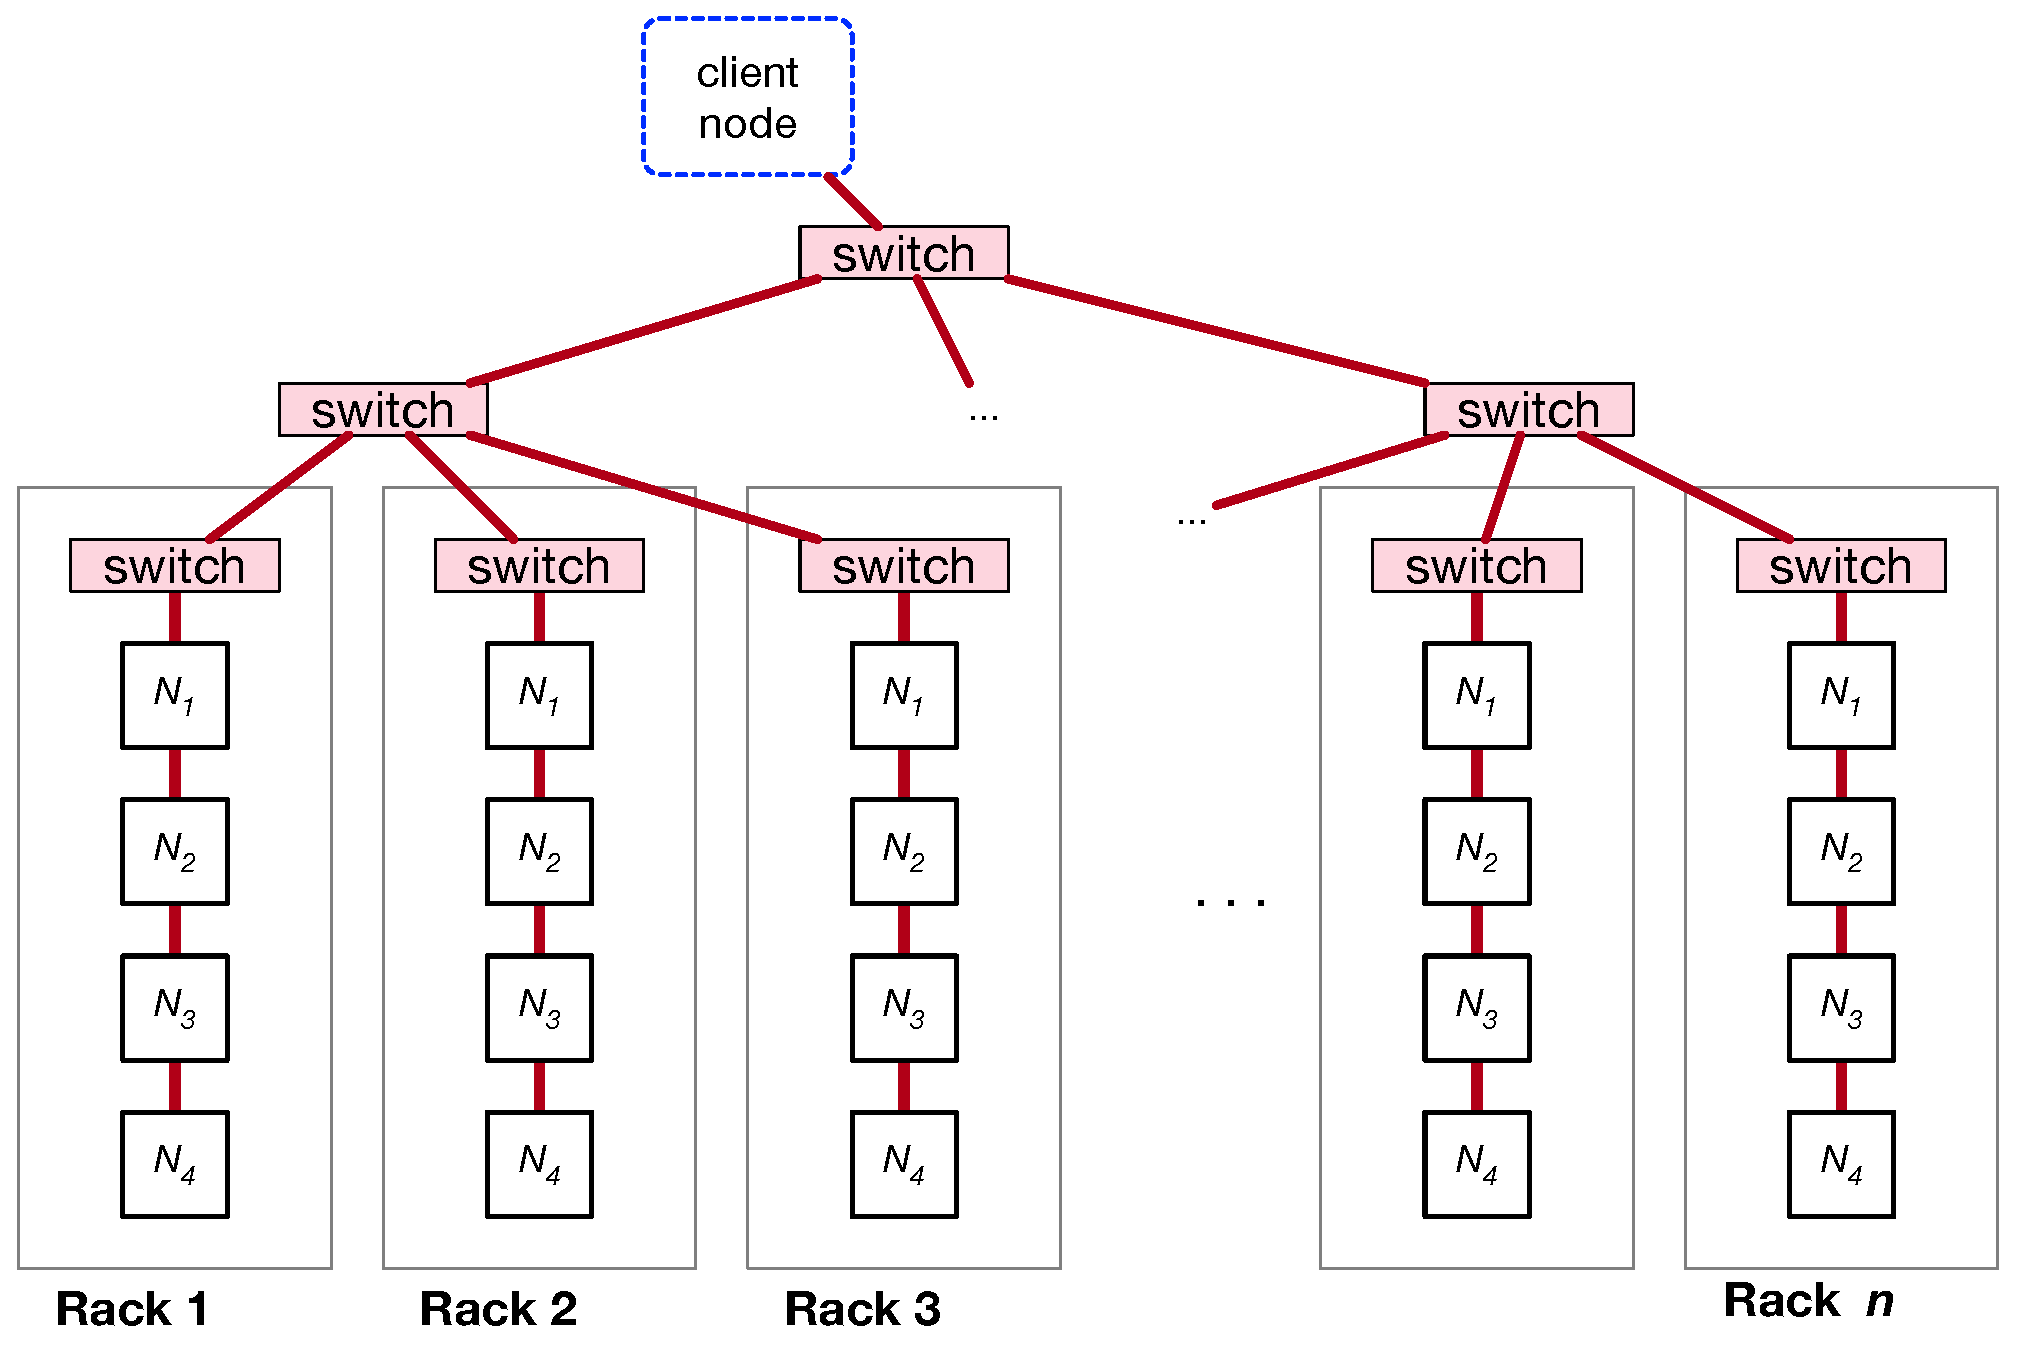
\includegraphics[width=0.75\textwidth]{figures/map_reduce_racks.eps}
\end{center}

We now look into using a shared-nothing cluster as a parallel computer for data processing.
\end{frame}

%
% ----------------------------------------------------------------------------------------------------
%


\begin{frame}

Map/Reduce is a functional programming paradigm that can be easily parallelized.

Very popular inside Google from 2004:
{\footnotesize\url{https://research.google.com/archive/mapreduce-osdi04-slides/index.html}}

Facebook and Yahoo both invested in the open source Apache Hadoop project\\
{\footnotesize{\url{https://wiki.apache.org/hadoop/PoweredBy\#F}}}\\
{\footnotesize{\url{https://wiki.apache.org/hadoop/PoweredBy\#Y}}}\\

\end{frame}


%
% ----------------------------------------------------------------------------------------------------
%


\begin{frame}{HDFS: Redundancy and Load Balancing}

Each blocks of a file is replicated (usually twice) across nodes and across racks (to account for network component failures).

The ``directory'' is kept by a ``name node'' (in Hadoop terminology), which tells the client which nodes have the data.

Any node with the data can process it.

\begin{center}
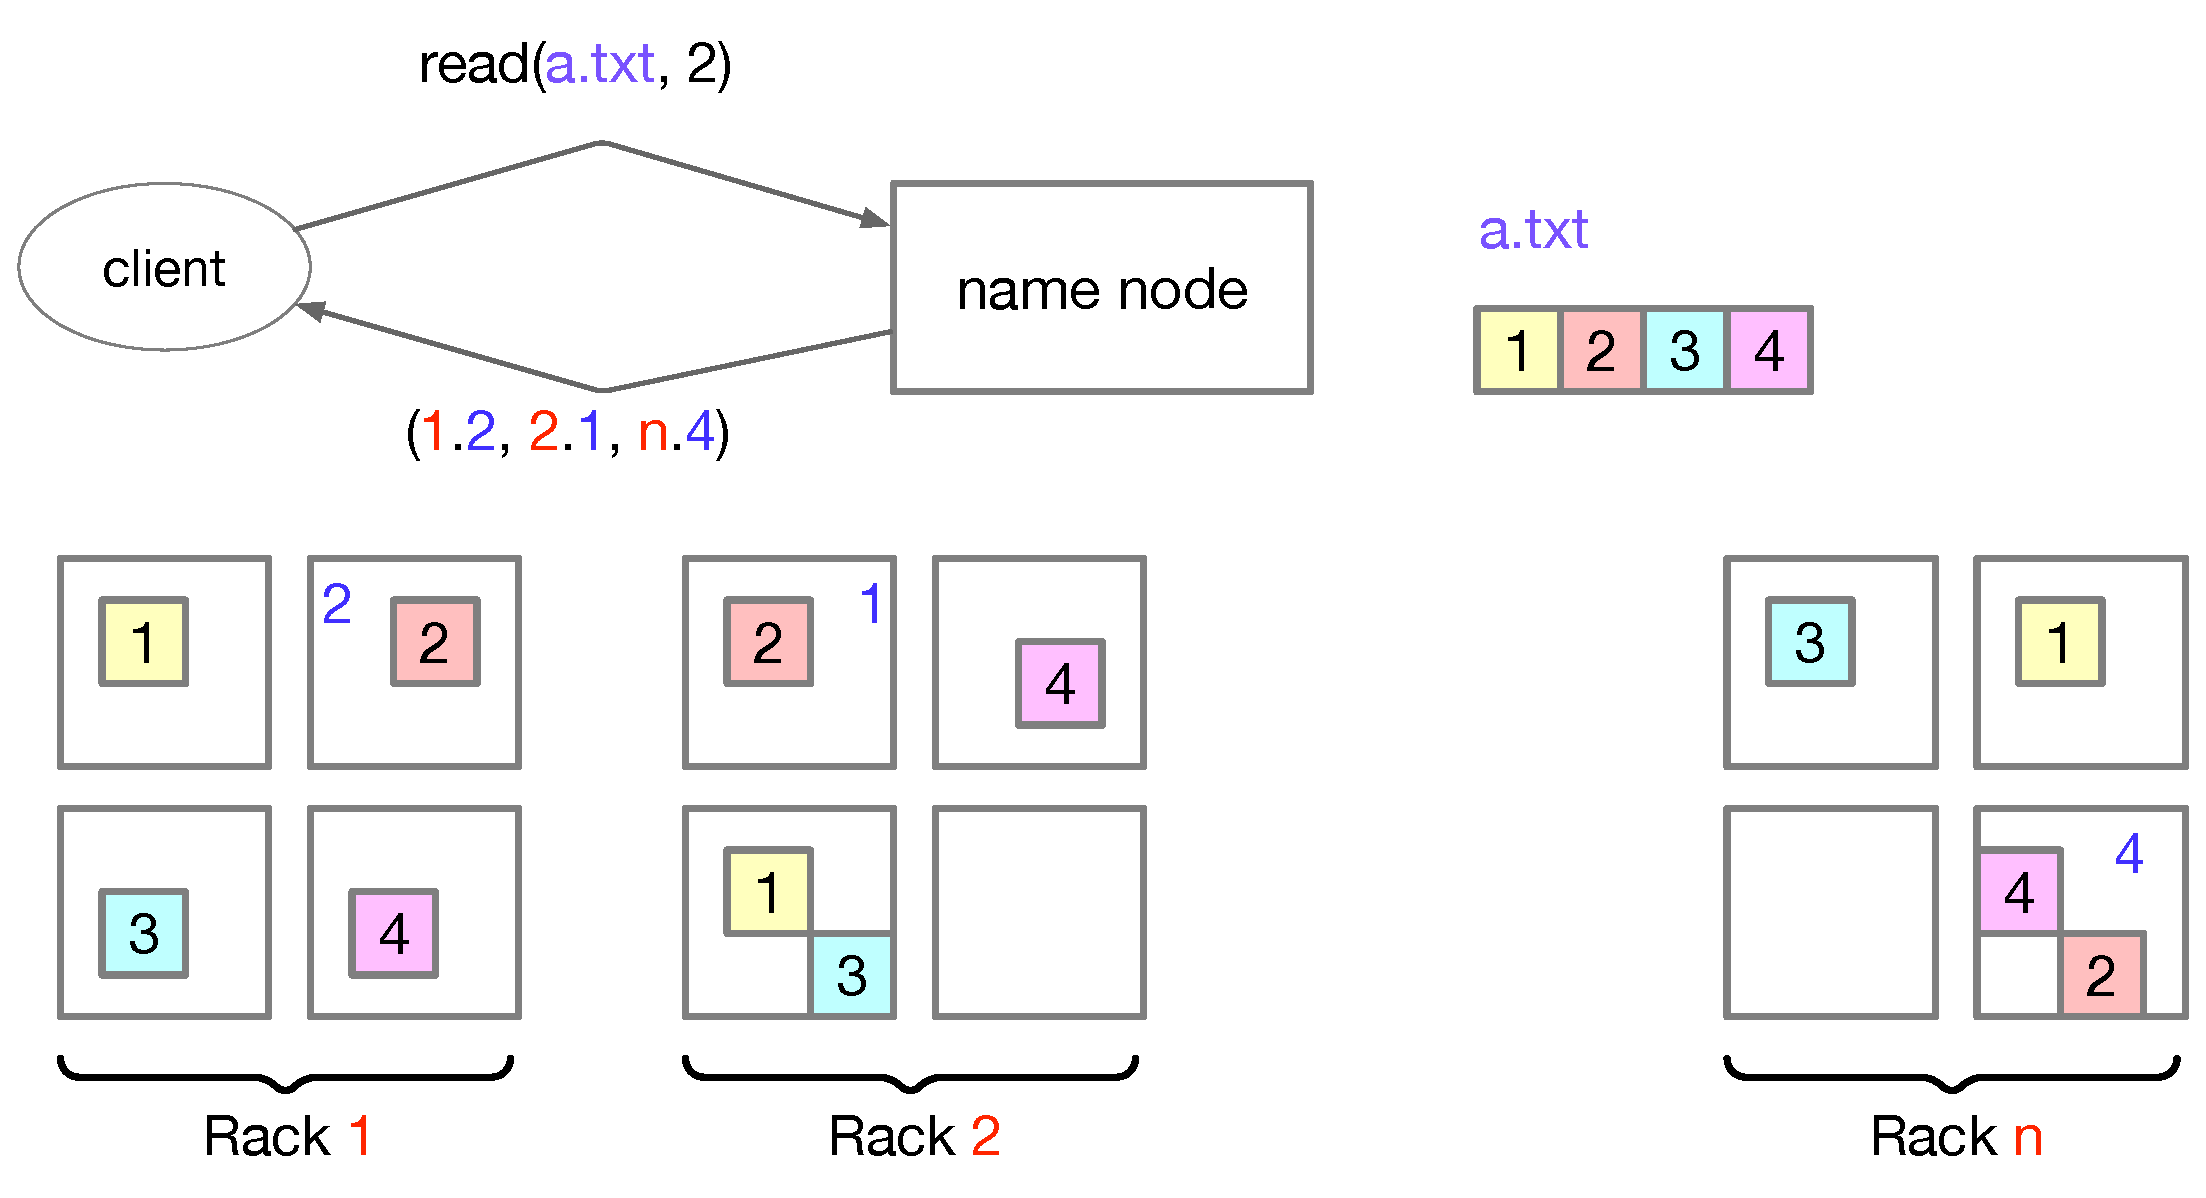
\includegraphics[width=0.75\textwidth]{figures/hdfs_blocks.eps}
\end{center}

\end{frame}

%
% ----------------------------------------------------------------------------------------------------
%


\begin{frame}{Programming Parallel Computers is Hard}

\blue{\textbf{Challenge \#1}}: it is hard to design the control flow when multiple computations happen \emph{at the same time} and in different computing nodes...
\begin{itemize}[-]
\item It is \textbf{very hard} to debug such designs.
\end{itemize}

\blue{\textbf{Challenge \#2}}: giving the programmers a  \alert{programming paradigm} simple enough so that we can easily express computations, yet \textbf{powerful enough} to be practical.

\vskip1em

\begin{block}{}
\alert{MapReduce} is a simple functional and powerful programming paradigm. Computations in MapRedure are:
\begin{itemize}[-,noitemsep]
\item easy to understand by humans
\item can be executed in parallel in massive clusters
\end{itemize}
\end{block}

\end{frame}

%
% ----------------------------------------------------------------------------------------------------
%


\begin{frame}{Data locality is important}

The goal of using a cluster was to avoid the communication cost of moving all the data around.
\begin{itemize}[-]
\item Some communication is unavoidable, however.
\end{itemize}

Parallel programs often alternate between:
\begin{itemize}[-,noitemsep]
\item Computing with \emph{local data} (no communication).
\item Exchanging results of local computation with other nodes.
\end{itemize}


\blue{\textbf{Challenge \#3}}: avoiding ``all-to-all'' communication model where every node exchanges data with every other node

\begin{block}{}
\alert{MapReduce computations work in stages}: map operations work on local data, reduce operations aggregate results. Communications are directed.
\end{block}
\end{frame}

%
% ----------------------------------------------------------------------------------------------------
%


\begin{frame}

\vskip2em

\begin{block}{Stages of MapReduce computations}
\begin{itemize}[-,noitemsep]
\item map operations work on local data, and produce \alert{$\textit{key},\textit{value}$} tuples
\item tuples are grouped together by key
\item all tuples with \alert{the same key} are sent to the same reduce task
\end{itemize}
\end{block}

\vskip1em 

\begin{center}
\includegraphics[width=0.75\textwidth]{figures/mapreduce_workflow.png}
\end{center}
\end{frame}


%
% ----------------------------------------------------------------------------------------------------
%

\begin{frame}{Execution of a MapReduce job}
\begin{center}
\includegraphics[width=0.65\textwidth]{figures/mapreduce_forking.png}
\end{center}

\vspace*{-1em}

The program specifies the \lstinline{map()} and \lstinline{reduce()} functions 

The \myblue{Master} process starts ``worker'' processes to complete all \lstinline{map()} tasks; once they are done, the \myblue{Master} starts ``workers'' for the \lstinline{reduce()} tasks.

\end{frame}


%
% ----------------------------------------------------------------------------------------------------
%


\begin{frame}[fragile]{Word count with MapReduce}

Suppose we want to \alert{count the number of times each word appears} in a large corpus of texts (e.g., millions of documents).
\begin{itemize}[-,noitemsep]
\item Each compute node has many documents in its local storage
\item No compute node has all occurrences of any single word
\end{itemize}

\vskip2em

General idea:
\begin{enumerate}[(1),noitemsep]
\item \alert{Map}: emit tuples \myblue{$(w,1)$} for every occurrence of a word in a document
\item \alert{Group} all streams of tuples with the same word
\item \alert{Reduce}: return tuple \myblue{$(w, l)$} where \myblue{$l$} is the number of tuples for word \myblue{$w$}
\end{enumerate}

\end{frame}

%
% ----------------------------------------------------------------------------------------------------
%


\begin{frame}[fragile]

\begin{block}{Map operation}
For every file \myred{\emph{f}} stored locally, do:
\begin{itemize}[-]
\item normalize and tokenize \myred{\emph{f}} into a list of words \lstinline[mathescape]![w$_1$, w$_2$, $\ldots$, w$_n$]!
\item for every word \myred{\emph{w}} in \lstinline[mathescape]![ w$_1$, w$_2$, $\ldots$, w$_n$]!
\begin{itemize}[$\rightarrow$]
\item \alert{emit} tuple \lstinline[mathescape]!(w, 1)!
\end{itemize}
\end{itemize}
\end{block}

\vskip1em

\begin{block}{Reduce operation}
\textbf{Input}: stream of tuples $t_1=(w_j, 1), t_2=(w_j,1),\ldots, t_k=(w_j,1)$\\
\textbf{Output}: \alert{$k$}
\end{block}

\vskip1em

Where does the output go?

The reduce operation can write data to a file. So, each compute node could open a file for each word it received...
\end{frame}


%
% ----------------------------------------------------------------------------------------------------
%


\begin{frame}{Execution of a MapReduce job}
\begin{center}
\includegraphics[width=0.65\textwidth]{figures/mapreduce_forking.png}
\end{center}

\vspace*{-1em}

The program specifies the \lstinline{map()} and \lstinline{reduce()} functions 

The \myblue{Master} process starts ``worker'' processes to complete all \lstinline{map()} tasks; once they are done, the \myblue{Master} starts ``workers'' for the \lstinline{reduce()} tasks.

\end{frame}


%
% ----------------------------------------------------------------------------------------------------
%


\begin{frame}
\centering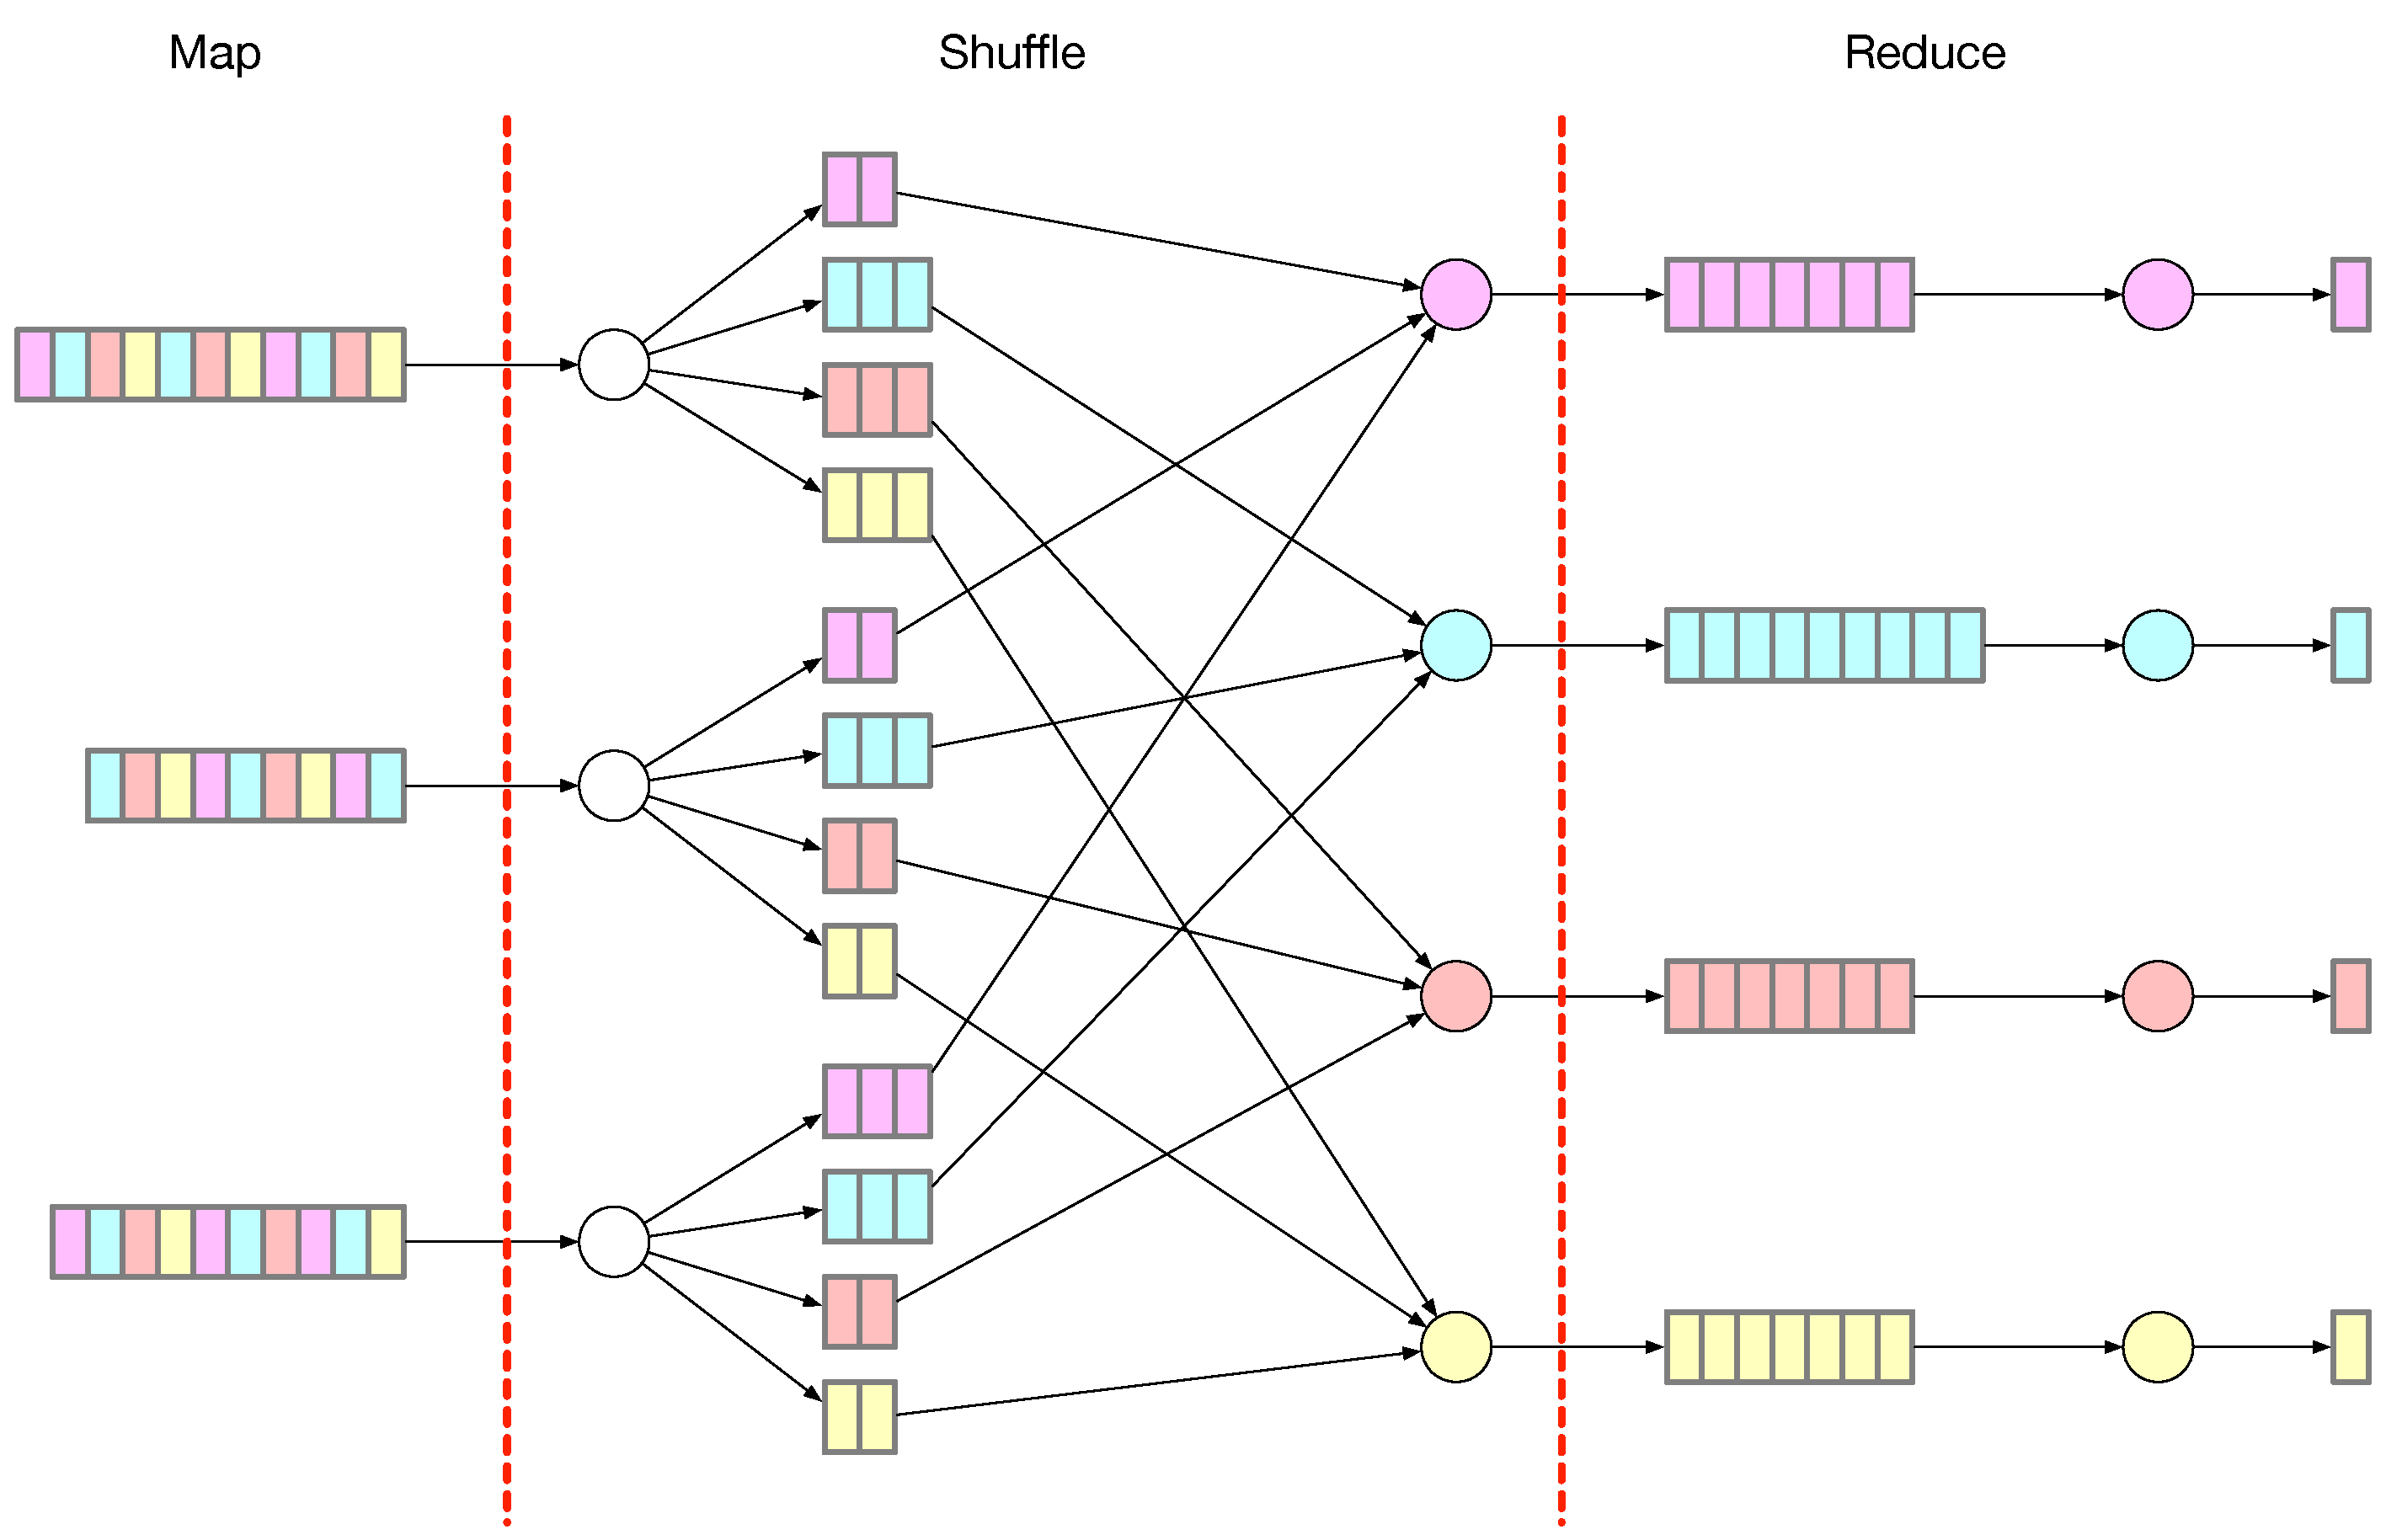
\includegraphics[width=\textwidth]{figures/map_reduce_shuffle.eps}
\end{frame}


%
% ----------------------------------------------------------------------------------------------------
%


\begin{frame}{Networking Cost}

\begin{center}
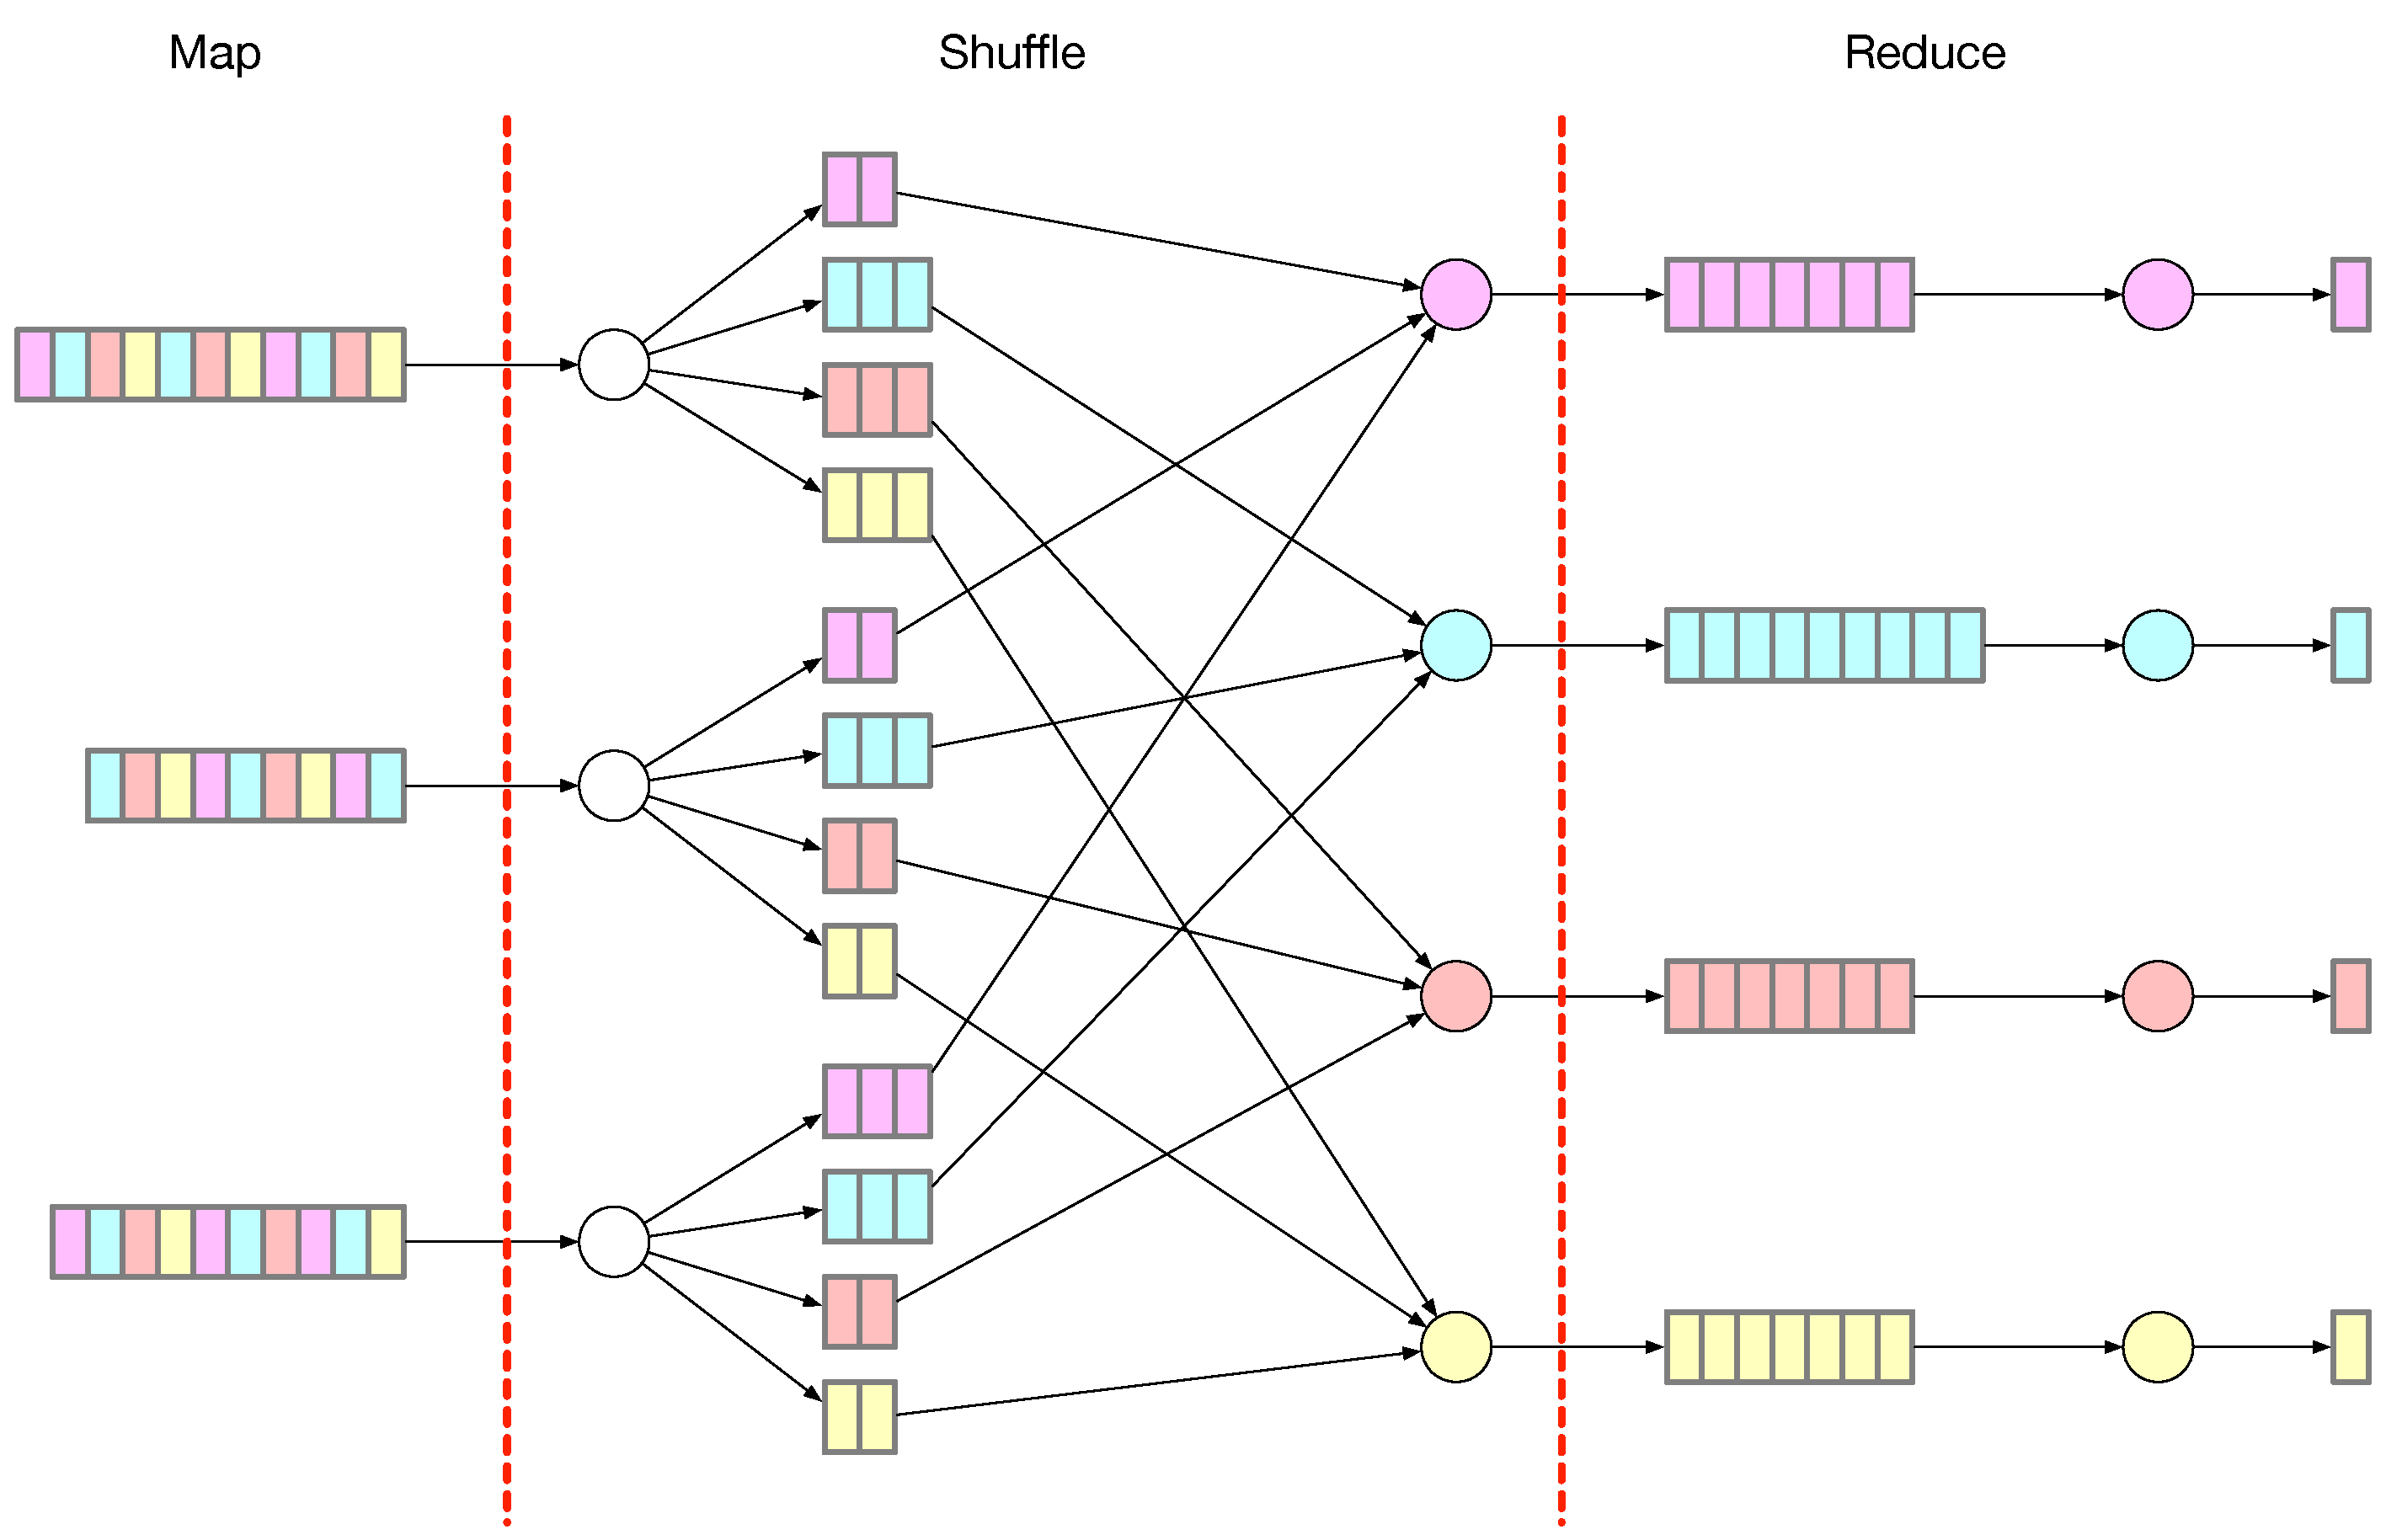
\includegraphics[width=0.5\textwidth]{figures/map_reduce_shuffle.eps}
\end{center}

The master assigns keys to nodes, deciding which nodes will perform which \lstinline{reduce()} operations.

Then, the nodes ``shuffle'' the stream of tuples, sending each tuple to the right \lstinline{reduce()} node.

\alert{\textbf{NOTE THAT} each node keeps at least one list of tuples though!}
\end{frame}


%
% ----------------------------------------------------------------------------------------------------
%


\begin{frame}{Obvious optimization}

The example so far is the ``textbook'' word count, where each tuple has count 1 for every word. 

An obvious optimization would be for the \lstinline!map()! operation to emit \alert{one tuple per word} among all documents it reads. This is possible, of course, only if the computing node has enough RAM to keep that map in memory.

\vskip1em

But even if the node does not have a lot of memory, it can keep accumulating word counts until all RAM is used up. At that point, the node can emit all tuples and start counting again.

\end{frame}

%
% ----------------------------------------------------------------------------------------------------
%


\begin{frame}{Multi-stage computations}

It is possible to have more complex computations involving several MapReduce phases. Below is one example MapReduce computation following finding individual word counts. 

Note that each node is left with a list of tuples, each with the count of an individual word, and that no two nodes have the count of the same word.

\vskip1em

\alert{Finding total number of words:}

\begin{block}{\lstinline{map()}}
Go over all words in the node and \alert{emit} a single tuple (\emph{\myblue{k}},\myred{\emph{total}}) where total is the sum of individual word counts in the node.
\end{block}

\begin{block}{\lstinline{reduce()} -- note that all tuples have the same key \myblue{\emph{k}}}
Sum up the values in the incoming tuples.
\end{block}
\end{frame}


%
% ----------------------------------------------------------------------------------------------------
%


\begin{frame}

\alert{Finding word(s) with highest frequency:}

\begin{block}{\lstinline{map()}}
Go over all word counts in the node; \alert{emit} a single tuple \lstinline[mathescape]!($k$,($c$,(w$_1$, w$_2$, $\ldots$, w$_n$)))! where:
\begin{itemize}[-,noitemsep]
\item $k$ is any constant
\item $c$ is the highest word frequency among all words in the node
\item \lstinline[mathescape]!w$_1$, w$_2$, $\ldots$, w$_n$! are all the words with count $c$
\end{itemize}
\end{block}

\begin{block}{\lstinline{reduce()} -- note that all tuples have the same key \myblue{\emph{k}}}
Go over the stream of tuples; find the highest count; return all words with that count.
\end{block}

Note that the highest count can be found in multiple nodes... so the reducer may have to merge word lists coming from different mappers.
\end{frame}

%
% ----------------------------------------------------------------------------------------------------
%


\begin{frame}{Matrix Operations in Map/Reduce}

Google's PageRank algorithm can be elegantly stated and efficiently computed as a series of matrix multiplications, which they implemented using Map Reduce for scalability reasons.

In fact, Google was probably among the first company to build a fortune on linear algebra.

Let $A$ be a $m\times n$ matrix (e.g., the adjacency matrix of the Web graph), and $\vec{v}$ be an $n$-dimensional vector.

\begin{block}{Vector-matrix product $x_i=\displaystyle\sum_{j=1}^{n}a_{ij}v_j$}
\begin{itemize}[-,noitemsep]
\item \lstinline{map()}: taking the entire $\vec{v}$ as input, compute $a_{ij}v_j$ for all cells of the matrix stored at the node; emit tuple $(i, m_{ij}v_j)$.
\item \lstinline{reduce()}: sum all partial values of $a_{ij}v_j$ for each key $i_x$, and write $i_x$ and the sum to the output.
\end{itemize}
\end{block}
\end{frame}

%
% ----------------------------------------------------------------------------------------------------
%


\begin{frame}

Let $A$ be a $m\times p$ matrix $B$ be an $p\times n$ matrix. 

The \alert{product} $AB$ is the $m \times n$ matrix $C$, in which element $c_{ij} = \displaystyle\sum_{k} a_{ik}b_{kj}$ and 

One way to compute $C$ is through two map/reduce stages:



\begin{block}{Matrix Multiplication Stage 1}
\begin{itemize}[-,noitemsep]
\item \lstinline{map()}: emit each matrix element for whatever matrix data is in the node. That is, emit all $(k,(A, i, a_{ik}))$ and $(k,(B, j, b_{kj}))$.
\item \lstinline{reduce()}: for each pair $(A, i, a_{ik})$ and $(B, j, b_{kj})$ that agree on the same $k$, write the tuple $(k,i,j,a_{ik}b_{kj})$.
\end{itemize}
\end{block}

At the end Stage 1, we can build a separate list for each value of $k$: $(i_1, j_1, v_1), (i_2, j_2, v_2), \ldots, ((i_p, j_p), v_p)$ with all combinations of $i,j$ and factors whose sum that will go into cell $c_{ij}$.
\end{frame}

%
% ----------------------------------------------------------------------------------------------------
%


\begin{frame}

The first stage computes, effectively lists of the form

\[(k, [(i_1, j_1, v_1), (i_2, j_2, v_2), \ldots, ((i_p, j_p), v_p)] \]

In this stage we compute an \emph{aggregate} (the sum) of these lists.

\vskip1em

\begin{block}{Matrix Multiplication Stage 2}
\begin{itemize}[-,noitemsep]
\item \lstinline{map()}: go through the tuples from the previous stage and emit $((i_1,j_1), v_1), ((i_1, j_1), v_2), \ldots ((i_p, j_p), v_p)$.
\item \lstinline{reduce()}: sum up all values with the same $(i,j)$, and write $((i,j) \displaystyle\sum_{p}v_p)$ to the final output.
\end{itemize}
\end{block}
\end{frame}

\def\MRclusterExample{
\draw (0,2) rectangle (1.5,3.5);
\node (n1t1) at (0,3.5) [anchor=north west] {\lstinline!R(1,2)!};
\node (n1t2) [below=0em of n1t1] {\lstinline!R(2,1)!};
\node (n1t3) [below=0em of n1t2] {\lstinline!S(1,2)!};
\node [left=0.0125cm of n1t1] {\small $N_1$};

\draw (0,0) rectangle (1.5,1.5);
\node (n2t1) at (0,1.5) [anchor=north west] {\lstinline!R(4,2)!};
\node (n2t2) [below=0em of n2t1] {\lstinline!R(5,2)!};
\node (n2t3) [below=0em of n2t2] {\lstinline!S(3,2)!};
\node [left=0.0125cm of n2t1] {\small $N_2$};

\draw (2.5,2) rectangle (4,3.5);
\node (n3t1) at (2.5,3.5) [anchor=north west] {\lstinline!R(3,1)!};
\node (n3t2) [below=0em of n3t1] {\lstinline!S(2,1)!};
\node [left=0.0125cm of n3t1] {\small $N_3$};

\draw (2.5,0) rectangle (4,1.5);
\node (n4t1) at (2.5,1.5) [anchor=north west] {\lstinline!S(3,3)!};
\node [left=0.0125cm of n4t1] {\small $N_4$};
}

\newsavebox{\MRdataset}
\savebox{\MRdataset}{\begin{tikzpicture}
\MRclusterExample
\end{tikzpicture}}

\section{Relational Operators with Map/Reduce}

%
% ----------------------------------------------------------------------------------------------------
%


\begin{frame}{Relational Operators with Map Reduce}

All basic relational operators can be easily implemented with Map/Reduce reading from a relational store in each cluster node\footnote{Apache's Pig \url{https://pig.apache.org} is a fairly powerful SQL-on-map-reduce.}.

Example dataset, with schema $R(a,b),\ \ S(c,d)$.

\vskip1em

\begin{center}
\usebox{\MRdataset}
\end{center}

\vskip1em
~
\end{frame}

%
% ----------------------------------------------------------------------------------------------------
%


\begin{frame}

\vskip2em

\begin{block}{Selection \alert{$\sigma_C R$} with a single reducer.}
\begin{itemize}[-,noitemsep,topsep=-10pt]
\item \lstinline!map()!: go through every tuple in the node, emit each tuple satisfying the selection with reduce key $k$.
\item \lstinline!reduce()!: collect all tuples.
\end{itemize}
\end{block}

Example: $\sigma_{b=1} R$

\begin{center}
\scalebox{0.75}{
\begin{tikzpicture}
\MRclusterExample
\node (reduce) at (8,2) [blue,cloud, draw,cloud puffs=10,cloud puff arc=120, aspect=2.5, inner sep=2pt] {reduce};
\draw [draw=red,->,>=stealth] (1,3.5) to[out=35,in=145] node[above]{\footnotesize  $(k, (2,1))$} (reduce);
\draw [draw=red,->,>=stealth] (4,2.5) to node[above]{\footnotesize  $(k, (3,1))$} (reduce);
\node (answer) [below right= 1cm and 0.125cm of reduce] {\footnotesize $[(2,1),(3,1)]$};
\draw[blue,->,>=stealth] (reduce) -- (answer);
\end{tikzpicture}}
\end{center}
\end{frame}


%
% ----------------------------------------------------------------------------------------------------
%


\begin{frame}
\vskip2em

\begin{block}{Projection \alert{$\pi_{a_i,\ldots, a_j} R$} with a single reducer.}
\begin{itemize}[-,noitemsep,topsep=-10pt]
\item \lstinline!map()!: go through every tuple in the node; collect all projected tuples; emit tuple $(k, [(v_1), (v_2), \ldots, (v_x)])$  with unique projected tuples.
\item \lstinline!reduce()!: gather all tuple streams!.
\end{itemize}
\end{block}

\begin{columns}[onlytextwidth]
\begin{column}{0.25\textwidth}
Example: $\pi_{b} R$
\end{column}
\begin{column}{0.8\textwidth}
\scalebox{0.75}{
\begin{tikzpicture}
\MRclusterExample
\node (reduce) at (8,2) [blue,cloud, draw,cloud puffs=10,cloud puff arc=120, aspect=2.5, inner sep=2pt] {reduce};
\draw [draw=red,->,>=stealth] (1,3.5) to[out=35,in=145] node[above]{\footnotesize  $(k, [(2),(1)])$} (reduce);
\draw [draw=red,->,>=stealth] (4,2.5) to node[above]{\footnotesize  $(k, [(1)])$} (reduce);
\draw [draw=red,->,>=stealth] (1,0) to[out=345,in=225] node[below]{\footnotesize  $(k, [(2)])$} (reduce);
\node (answer) [below right= 1cm and 0.125cm of reduce] {\footnotesize $[(1),(1),(2),(2)]$\footnotemark};
\draw[blue,->,>=stealth] (reduce) -- (answer);
\end{tikzpicture}}
\end{column}
\end{columns}


\footnotetext{Recall that the SQL version of project does not remove duplicates.}
\end{frame}

%
% ----------------------------------------------------------------------------------------------------
%


\begin{frame}{Set Operations}

General idea: every mapper emits each original tuple as the (reduce) key and the relation name as the value.

\vskip1em
\begin{columns}[onlytextwidth]
\begin{column}{0.33\textwidth}
In our example, this would produce the streams to the right.
\vskip1em
The reducer implements the set operator.
\end{column}
\begin{column}{0.65\textwidth}
\scalebox{0.75}{
\begin{tikzpicture}
\node (reduce1) at (0,0) [blue,cloud, draw,cloud puffs=10,cloud puff arc=120, aspect=2.5, inner sep=2pt] {reduce};
\node (input1) [left=1.25cm of reduce1] {$((1,2), R), ((1,2), S)$};
\node (answer1) [right= 0.5cm of reduce1,text width=1cm] {\footnotesize $[\ \ldots\ ]$};
\draw[->,>=stealth] (input1) -- (reduce1);
\draw[blue,->,>=stealth] (reduce1) -- (answer1);

\node (reduce2) [below=5pt of reduce1] [blue,cloud, draw,cloud puffs=10,cloud puff arc=120, aspect=2.5, inner sep=2pt] {reduce};
\node (input2) [left=1.25cm of reduce2] {$((2,1), R), ((2,1), S)$};
\node (answer2) [right= 0.5cm of reduce2,text width=1cm] {\footnotesize $[\ \ldots\ ]$};
\draw[->,>=stealth] (input2) -- (reduce2);
\draw[blue,->,>=stealth] (reduce2) -- (answer2);

\node (reduce3) [below=5pt of reduce2] [blue,cloud, draw,cloud puffs=10,cloud puff arc=120, aspect=2.5, inner sep=2pt] {reduce};
\node (input3) [left=1.25cm of reduce3] {$((3,1), R)$};
\node (answer3) [right= 0.5cm of reduce3,text width=1cm] {\footnotesize $[\ \ldots\ ]$};
\draw[->,>=stealth] (input3) -- (reduce3);
\draw[blue,->,>=stealth] (reduce3) -- (answer3);

\node (reduce4) [below=5pt of reduce3] [blue,cloud, draw,cloud puffs=10,cloud puff arc=120, aspect=2.5, inner sep=2pt] {reduce};
\node (input4) [left=1.25cm of reduce4] {$((3,2), S)$};
\node (answer4) [right= 0.5cm of reduce4,text width=1cm] {\footnotesize $[\ \ldots\ ]$};
\draw[->,>=stealth] (input4) -- (reduce4);
\draw[blue,->,>=stealth] (reduce4) -- (answer4);

\node [below of=reduce4, rotate=90] {...};
\end{tikzpicture}}
\end{column}
\end{columns}

\begin{itemize}[-,noitemsep]
\item \alert{$R\cap S$}: reducer keeps keys with both values.
\item \alert{$R\cup S$}: reducer keeps all unique keys.
\item \alert{$R-S$}: reducer keeps keys with value $R$ but not $S$.
\end{itemize}
\end{frame}

%
% ----------------------------------------------------------------------------------------------------
%


\begin{frame}
\vskip2em

\begin{block}{Join \alert{$R \Join_{x=y} S$}}
\begin{itemize}[-,noitemsep,topsep=-10pt]
\item \lstinline!map()!: emit tuples from $R$ with attribute $R.x$ as key, and tuples from $S$ with $S.y$ as key.
\item \lstinline!reduce()!: iterate through the incoming lists with matching values!
\end{itemize}
\end{block}

Example: $R \Join_{b=c} S$

\begin{center}
\scalebox{0.75}{
\begin{tikzpicture}
\MRclusterExample
\node (reduce1) at (8,3.75) [blue,cloud, draw,cloud puffs=10,cloud puff arc=120, aspect=2.5, inner sep=2pt] {reduce};
\draw [draw=red,->,>=stealth] (1,3.5) to[out=35,in=175] node[above,yshift=1pt]{\footnotesize $(1, (R, (2,1))), (1, (S, (1,2)))$} (reduce1);
\draw [draw=orange,->,>=stealth] (4,3.25) to[out=15,in=200] node[above]{\footnotesize $(1, (R, (3,1)))$} (reduce1);
\node (answer1) [right= 0.5cm of reduce1] {\footnotesize $[(2,1,1,2),\ (3,1,1,2)]$};
\draw[blue,->,>=stealth] (reduce1) -- (answer1);

\node (reduce2) at (8,1.5) [blue,cloud, draw,cloud puffs=10,cloud puff arc=120, aspect=2.5, inner sep=2pt] {reduce};
\draw [draw=red,->,>=stealth] (1.5,2.125) to[out=345,in=170] node[above,xshift=40pt]{\footnotesize $(2, (R, (1,2)))$} (reduce2);
\draw [draw=orange,->,>=stealth] (4,2.75) to[out=350,in=145] node[above,yshift=-1pt]{\footnotesize $(2, (S, (2,1)))$} (reduce2.north);
\draw [draw=green,->,>=stealth] (1.5,1.4) to[out=15,in=180] node[below,yshift=-3pt,xshift=25pt,text width=1cm]{\footnotesize $(2, (R, (4,2))),$ $(2, (R, (5,2)))$} (reduce2);
\node (answer2) [right= 0.5cm of reduce2,text width=1cm] {\footnotesize $[(1,2,2,1),\ (4,2,2,1)$ $(5,2,2,1)]$};
\draw[blue,->,>=stealth] (reduce2) -- (answer2);


\node (reduce3) at (8,-0.25) [blue,cloud, draw,cloud puffs=10,cloud puff arc=120, aspect=2.5, inner sep=2pt] {reduce};
\draw [draw=green,->,>=stealth] (1.25,0) to[out=345,in=185] node[below,xshift=-60pt,yshift=5pt]{\footnotesize $(3, (S, (3,2)))$} (reduce3);
\draw [draw=purple,->,>=stealth] (4,0.25) to[out=355,in=160] node[below,xshift=-10pt,yshift=-1pt]{\footnotesize $(3, (S, (3,3)))$} (reduce3);
\node (answer3) [right= 0.5cm of reduce3,text width=1cm] {\footnotesize $[\ \ ]$};
\draw[blue,->,>=stealth] (reduce3) -- (answer3);
\end{tikzpicture}}
\end{center}
\end{frame}

%
% ----------------------------------------------------------------------------------------------------
%


\begin{frame}{SQL in Map/Reduce}

Except for fixpoint-semantics recursion, pretty much all of SQL can be easily computed with Map/Reduce:
\begin{itemize}[-]

\item The ``bag'' versions of the set operations is also easily done in Map/Reduce: all that is needed is to count the number of (reduce) keys with value $R$ or $S$ in each stream.

\item Aggregations (\lstinline[style=SQL]!GROUP BY!) and set functions are also easily computable with Map/Reduce.

\item Duplicate elimination is also trivial when the reduce key is a tuple.
\end{itemize}
\end{frame}


\newsavebox{\mapreduceStepI}
\begin{lrbox}{\mapreduceStepI}
\begin{tikzpicture}
\MRclusterExample
%
\node (n4t2) [below=0em of n4t1] {\alert{\lstinline[style=cmput391]!-:t(2,1):-!}};
\node (n4t3) [below=0em of n4t2] {\alert{\lstinline[style=cmput391]!-:t(3,1):-!}};
%
\node (reduce) at (6.5,2) [blue,cloud, draw,cloud puffs=10,cloud puff arc=120, aspect=2.5, inner sep=2pt] {reduce};
\draw [draw=red,->,>=stealth] (1,3.5) to[out=45,in=135] node[above]{\footnotesize  $(k, (2,1))$} (reduce);
\draw [draw=red,->,>=stealth] (4,2.5) to node[above]{\footnotesize  $(k, (3,1))$} (reduce);
\draw[densely dotted,purple,->,>=stealth] (reduce) to[out=250, in=10] (4,0.5);
\end{tikzpicture}
\end{lrbox}

\newsavebox{\mapreduceStepII}
\begin{lrbox}{\mapreduceStepII}
\begin{tikzpicture}
\MRclusterExample
%
\node (n4t2) [below=0em of n4t1] {\alert{\lstinline[style=cmput391]!-:t(2,1):-!}};
\node (n4t3) [below=0em of n4t2] {\alert{\lstinline[style=cmput391]!-:t(3,1):-!}};
%
\node (reduce) at (6.5,2) [blue,cloud, draw,cloud puffs=10,cloud puff arc=120, aspect=2.5, inner sep=2pt] {reduce};
\draw [draw=red,->,>=stealth] (4,1) node[below right]{\footnotesize $(k, [(2),(3)])$} -- (reduce);
\node (answer) [below right= 1cm and 0.125cm of reduce] {\footnotesize $[(2),(3)]$};
\draw[blue,->,>=stealth] (reduce) -- (answer);
\end{tikzpicture}
\end{lrbox}



%
% ----------------------------------------------------------------------------------------------------
%


\begin{frame}{Multi-operator Queries}

We answer a query like $\pi_{a_1,\ldots,a_n}(\sigma_C(R))$ in two map/reduce processes:
\begin{enumerate}[(1),noitemsep]
\item Materialize $\text{\lstinline!t!} \leftarrow\sigma_C(R)$ in a temporary table.
\item Compute $\pi_{a_1,\ldots,a_n}(\text{\lstinline!t!})$ over the temporary table.
\end{enumerate}

\begin{center}
\scalebox{0.6}{
\begin{tikzpicture}
\node at (0,5.25) [blue] {step 1};
\node at (0,0) [anchor=south] {\usebox{\mapreduceStepI}};
\node at (9.5,5.25) [blue] {step 2};
\node at (9.5,0) [anchor=south] {\usebox{\mapreduceStepII}};
\end{tikzpicture}}
\end{center}

\end{frame}


%
% ----------------------------------------------------------------------------------------------------
%


\begin{frame}{How many reducers to use?}

Recall that in every map/reduce computation:
\begin{itemize}[-,noitemsep]
\item The number of \lstinline!map()! tasks is the same as the number of computing nodes.
\item The number of \lstinline!reduce()! tasks is the same \textbf{as the number} of reduce keys!
\end{itemize}

\vskip1em

\begin{block}{Why does this matter?}
If the first step uses a single reducer:
\begin{itemize}[-,noitemsep]
 \item A single node will store all tuples from the first step\footnotemark.
 \item Only one \lstinline!map()! task will run in the second step.
\end{itemize}
\end{block}
\footnotetext{Of course, the cluster may be setup to replicate the data across multiple nodes, alleviating the problem.}
\end{frame}


%
% ----------------------------------------------------------------------------------------------------
%


\begin{frame}

\vskip2em

\begin{block}{Selection \alert{$\sigma_C R$} with \textbf{multiple} reducers.}
\begin{itemize}[-,noitemsep,topsep=-10pt]
\item \lstinline!map()!: go through every tuple in the node, emit each tuple satisfying the selection using the tuple itself\footnotemark as key.
\item \lstinline!reduce()!: collect all copies of each tuple.
\end{itemize}
\end{block}

Example: $\sigma_{b=1} R$

\begin{center}
\scalebox{0.75}{
\begin{tikzpicture}
\MRclusterExample
\node (reduceA) at (8.5,3) [blue,cloud, draw,cloud puffs=10,cloud puff arc=120, aspect=2.5, inner sep=2pt] {reduce};
\node (reduceB) at (8.5,1.5) [blue,cloud, draw,cloud puffs=10,cloud puff arc=120, aspect=2.5, inner sep=2pt] {reduce};
\draw [draw=red,->,>=stealth] (1,3.5) to[out=35,in=175] node[above]{\footnotesize  $((2,1), (2,1))$} (reduceA);
\draw [draw=red,->,>=stealth] (4,2.5) to[out=325,in=180] node[above,xshift=20pt]{\footnotesize  $((3,1), (3,1))$} (reduceB);
\node (answerA) [right= 0.5cm of reduceA] {\footnotesize $[(2,1)]$};
\node (answerB) [right= 0.5cm of reduceB] {\footnotesize $[(3,1)]$};
\draw[blue,->,>=stealth] (reduceA) -- (answerA);
\draw[blue,->,>=stealth] (reduceB) -- (answerB);
\end{tikzpicture}}
\end{center}

\vskip1em 

\footnotetext{A hash of the tuple would also work, and save on communication costs.}

\end{frame}


%
% ----------------------------------------------------------------------------------------------------
%


\begin{frame}
How many reducers should one use?
\begin{itemize}[-]
\item A single reducer can intuitively act as the ``server-side'' transaction process for each request by a connected user/application.
\item With multiple reducers (which run as independent processes), one can spread the tuples in the ``temporary table'' across more nodes, increasing the number of \lstinline!map()! tasks that \textbf{run in parallel} in subsequent steps.
\item Thus, multiple reducers seem better for intermediate query operations, while the single reducer approach seems better for the root node of the query.
\end{itemize}
\end{frame}


%
% ----------------------------------------------------------------------------------------------------
%


\begin{frame}[fragile]{Map/Reduce in NoSQL systems}

Some document stores like CouchDB use Map/Reduce for parallel query processing~\footnote{\url{https://docs.couchdb.org/en/stable/ddocs/views/intro.html}}. 

For example, one can use \lstinline!map()! functions to select multiple (fragments) of JSON documents in the cluster that satisfy a predicate, querying all documents in the cluster simultaneously, and the \lstinline!reduce()! function to compute an aggregate answer.

\begin{columns}[onlytextwidth]
\begin{column}{0.5\textwidth}
\begin{lstlisting}[basicstyle=\ttfamily\scriptsize]
function map(doc) {
  if(doc.author.includes("Manning")) {
      emit(doc.publisher,
       doc.title);
  }
}
\end{lstlisting}
\end{column}
\quad\begin{column}{0.45\textwidth}
\begin{lstlisting}[basicstyle=\ttfamily\scriptsize]
function reduce(key, values) {
  var cnt = 0;
    for(var idx in values) {
      cnt = cnt + 1;
  }
  return (key, cnt);
}\end{lstlisting}
\end{column}
\end{columns}
\end{frame}

